We will be determining the collinear Lagrange points from a rotating frame of reference relative to a circular orbit of Earth.
This simplifies the solution to a single dimension which bisects the Sun and Earth. % ELABORATE

\vspace*{0.5cm}
\begin{figure}[!h]
	\centering
	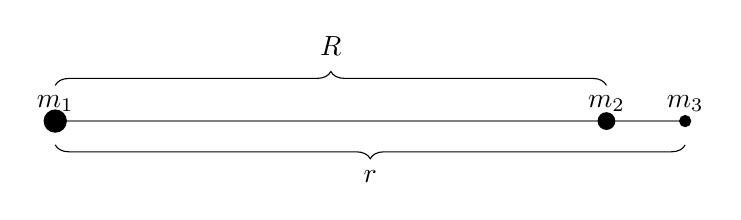
\begin{tikzpicture}
		\draw[gray,thick] (-4,0) -- (4,0);
		\filldraw (-4,0) circle (4pt) node[anchor=south]{$m_1$};
		\filldraw (3,0) circle (3pt) node[anchor=south]{$m_2$};
		\filldraw (4,0) circle (2pt) node[anchor=south]{$m_3$};
		\draw[decorate,decoration={brace,amplitude=5pt,raise=3ex}] (-4,0) -- (3,0) node[midway,yshift=27pt]{$R$};
		\draw[decorate,decoration={brace,mirror,amplitude=5pt,raise=2ex}] (-4,0) -- (4,0) node[midway,yshift=-2em]{$r$};
	\end{tikzpicture}
	\vspace*{0.25cm}
	\caption{Simple diagram of the Sun-Earth system.}
	\label{fig:collinear-coords}
\end{figure}

\textit{R} will be the distance between the Sun and Earth, while \textit{r} will be the distance from the main body to the Lagrange point. 
The masses of the Sun, Earth, and a point located at the Lagrange point are denoted by $m_1$, $m_2$, and $m_3$, respectively.
For the sake of maintaining direction, bodies positioned to the right will have a positive distance, and vice versa.

It is important to understand what factors are at play when dealing with Lagrange points.
What will be most important is Newton's Law of Gravitation,
\begin{equation}
	F = \frac{Gm_1m_2}{r^2}
\end{equation}
where \textit{F} is the force exerted between two bodies of mass, \textit{G} is the gravitational constant, m is the mass of a body, and \textit{r} is the distance between the two bodies.
%The sum of forces acting on our fictional object $m_3$ due to gravity is then
%\begin{equation}
%	F = -\frac{Gm_1m_3}{r^3} - \frac{Gm_2m_3}{(r-R)^3}
%\end{equation}
We must also consider the centrifugal and Coriolis forces acted on the object at the Lagrange point.
We can rule out the Coriolis force, since the collinear Lagrange points will not be moving in our rotating frame of reference.
As for centrifugal force, it will be proportional to the centripetal force,
\begin{equation*}
	F = m\omega^2r
\end{equation*}
where $\omega$ is the angular velocity of the object. Understanding that angular velocity can be defined as
\begin{equation*}
	\omega = \frac{2\pi}{T}
\end{equation*}
and the period of a circular orbit from Kepler's third law as
\begin{equation*}
	T = 2\pi\sqrt{\frac{R^3}{G(m_1+m_2)}} \text{,} % NOTE: this may require citation.
\end{equation*}
the equation for angular velocity simplifies to
\begin{equation*}
	\omega^2 = \frac{G(m_1+m_2)}{R^3} \text{.} % NOTE: Gravitational Parameter is the sum of the two major masses. Citation^^?
\end{equation*} % You should add details as to why we are evaluating the radial acceleration. THERE IS A DISCEPENCY IN THE ALGREBRA!
Therefore, the sum of forces acting on an object at a Lagrange point is
\begin{equation*}
	F = m_3a = -\frac{Gm_1m_3}{r^2} - \frac{Gm_2m_3}{(r - R)^2} + \frac{G(m_1+m_2)}{R^3}rm_3 \text{.}
\end{equation*}
Solving for a radial acceleration of 0, we get the formula:
\begin{equation*}
	0 = -\frac{Gm_1}{r^2} - \frac{Gm_2}{(r - R)^2} + \frac{G(m_1+m_2)}{R^3}r \text{.}
\end{equation*}
Most of the variables are known constants, with \textit{r} being the only unknown value which represents the distance of the Lagrange point from $m_1$.
It is worth noting that, with respect to direction, $r^2$ and $(r-R)^2$ will only reflect acceleration in the negative direction and will not be sufficient to tell us where L1 and L3 are.
To remedy this, the formula is rewritten as such to preserve the sign of $r$:
\begin{equation*}
	0 = -\frac{Gm_1}{r|r|} - \frac{Gm_2}{(r - R)|r - R|} + \frac{G(m_1+m_2)}{R^3}r \text{.}
\end{equation*}
%The sign of each term in the equation is important to represent which direction acceleration is being applied.
%If $m_3$ were positioned between $m_1$ and $m_2$, for example, than the term $-\frac{Gm_2}{(r-R^2)}$ should be positive to show that the acceleration caused by the gravity of $m_2$ is in the outward direction.
%However, for each of the gravity terms in our equation, $r^2$ and $(r-R)^2$ will always be positive regardless ...
Further simplification of the formula results in a rational function that is almost impossible to solve by hand, in part because the formula would involve significantly large values due to the constants used.
%Additionally, there exists the cyclical issue of acceleration being dependent on distance and distance vice versa.
Instead, the roots of the formula are solved for computationally.
\begin{figure}[h!]
	\centering
	\captionsetup[subfigure]{justification=centering}
	\begin{subfigure}[b]{0.4\textwidth}
		\centering
		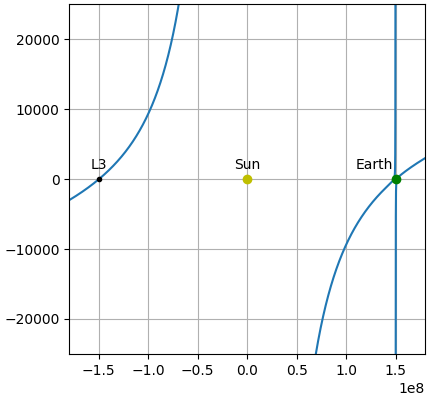
\includegraphics[scale=0.6]{r-accel-figure-1.png}
		\caption{\footnotesize Radial Acceleration between the Sun and Earth.}
		\label{fig:radial-accel-system}
	\end{subfigure}
	\hspace*{1cm}
	\begin{subfigure}[b]{0.4\textwidth}
		\centering
		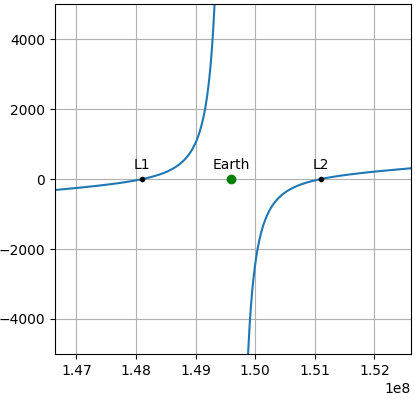
\includegraphics[scale=0.6]{r-accel-figure-2.png}
		\caption{\footnotesize Radial acceleration around the Earth.\vspace*{1.16em}}
		\label{fig:radial-accel-earth}
	\end{subfigure}
	\label{fig:radial-accel}
	\caption{Net acceleration of the Sun-Earth system. Graphs are created using \texttt{matplotlib}.}
\end{figure} % this figure can benefit from an explanation

%\begin{figure}[h!]
%	\centering
%	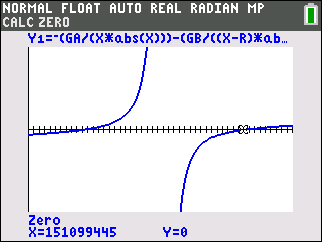
\includegraphics[scale=0.7]{accel-root.png}
%	\caption{Solution for L2 using a GDC.}
%	\label{fig:radial-l2}
%\end{figure}
Relative to the distance from the sun, the location of the Lagrange point L2 is $1.511\times10^8 \si{\kilo\metre}$.